\begin{frame}\begin{center}
\LARGE\textbf{Setup}
\end{center}\end{frame}



\begin{frame}
\textbf{Setup}

\medskip

Normal linear-in-parameters version of the generalized Roy model.

	\begin{align*}
	&\textbf{Potential Outcomes} & & \textbf{Choice}  &\\
	& Y_1 = \delta_1 X_i + U_{1} &  &D = \mathbf{1}\{\Phi(\gamma Z) > u_D\} &\\
	& Y_0 = \delta_0 X + U_{0} &  & \text{with $u_D = \Phi(V)$}  &\\
	&&&&\\
	&\textbf{Distributional Characteristics}&&&\\
	&\{U_{1}, U_{0}, V\} \sim \mathcal{N}\left(0, \Sigma\right)&&\Sigma =  \begin{bmatrix}
	\sigma_1^{2} & \sigma_{1,0} & \sigma_{1,V} \\
	\sigma_{1,0} & \sigma_0^{2} & \sigma_{0,V} \\
	\sigma_{1,V} & \sigma_{0,V} & \sigma_V^{2} \\
	\end{bmatrix}&\\
	&&&&\\
	& \textbf{Observed Outcome} &&&\\
	& Y_i = DY_1 + (1-D) Y_0 &&&
	\end{align*}
\end{frame}

\begin{frame}\begin{center}
\LARGE\textbf{Features}
\end{center}\end{frame}

\begin{frame}
\textbf{Features}

\medskip
\begin{itemize}\setlength\itemsep{1em}
\item \textit{grmpy} is currently capable of the following features:
\begin{itemize}\setlength\itemsep{1em}
  \item Simulating a dataset based on your own specifications.
  \item Providing some useful information about the simulated dataset for instance:

  \medskip
    \begin{itemize}\setlength\itemsep{1em}
    \item Distributional outcome characteristics
    \item $B^{ATE}, B^{TT}, B^{TUT}$
    \item $B^{MTE}$ by ventile
    \end{itemize}
  \item Estimating the coefficients of interest given a dataset (of a specific form).
\end{itemize}
\end{itemize}

\end{frame}

\begin{frame}
\textbf{Install the package}

\medskip
\begin{itemize}\setlength\itemsep{1em}
\item OS, Linux : Use the pip install manager (\textit{pip install grmpy}) or download the package via \href{https://github.com/OpenSourceEconomics/grmpy}{GitHub} and install it manually.
\item Windows:  The same procedure as for Linux, OS but you have to verify that the \textit{numpy} package is already installed on your machine.
\end{itemize}
\end{frame}

\begin{frame}
\textbf{Initialization file}

\medskip
\begin{itemize}\setlength\itemsep{1em}
\item The initialization file provides the user with the opportunity to specify all parameters of his/her model, for instance:\medskip
  \begin{itemize}\setlength\itemsep{1em}
  \item Simulation parameters (number of observations, name of the output files)
  \item Estimation parameters (optimization algorithm, start values)
  \item Optimizer spezifications
  \item Coefficients and covariance parameters, dummy variables ...
  \end{itemize}
\end{itemize}
\end{frame}

\begin{frame}
\textbf{Initialization file}

\medskip
\begin{itemize}
\item \href{examples/tutorial.grmpy.yml}{Example}
\item for a detailed explanation see: \href{http://grmpy.readthedocs.io/en/latest/tutorial.html}{\textit{grmpy}-documentation}
\end{itemize}
\vfill
\end{frame}

\begin{frame}
\textbf{Simulation}

\medskip
\begin{itemize}\setlength\itemsep{1em}
\item \textit{grmpy.simulate():}

\medskip
\begin{itemize}\setlength\itemsep{1em}
\item Input: path of the initialization file.
\item The function returns a data frame based on your specifications and different output files.

\medskip
\begin{itemize}\setlength\itemsep{1em}
\item The data set as a pickle and a txt file.
\item An \href{examples/data.grmpy.info}{Info file} that provides the distributional characteristics of the data as well as information about the different treatment effects.
\end{itemize}

\end{itemize}
\end{itemize}
\end{frame}

\begin{frame}
\textbf{Estimation}

\medskip
\begin{itemize}\setlength\itemsep{1em}
\item \textit{grmpy.fit():}\medskip
  \begin{itemize}\setlength\itemsep{1em}
  \item Input: path of the initialization file.
  \item At the moment the estimation process is only capable of two different optimization algorithms:

  \medskip
    \begin{itemize}\setlength\itemsep{1em}
    \item Broyden Fletcher Goldfarb Shanno (BFGS) algorithm
    \item  Powell's conjugate direction method
\end{itemize}
\end{itemize}
\end{itemize}

\end{frame}

\begin{frame}
\begin{itemize}\setlength\itemsep{1em}
\item There are two different options for the start values that could be set in the initialization file:\medskip
  \begin{itemize}\setlength\itemsep{1em}
  \item \textit{init:} The estimation process uses the coefficient values specified in the initialization file as the start values for the estimation process.
  \item \textit{auto:} The start values are determined via a simple OLS followed by a Probit regression for the choice indicator.
  \end{itemize}
  \item The estimation results are printed to an \href{examples/est.grmpy.info}{output file}.
\end{itemize}
\end{frame}

\begin{frame}
\textbf{Test battery}

\medskip
\begin{itemize}\setlength\itemsep{1em}
\item We also provide a test battery that includes several tests to ensure that the processes perform as intended.\medskip
\begin{itemize}\setlength\itemsep{1em}
\item Property-based testing
\item Reliability testing
\item Regression testing
\end{itemize}
\end{itemize}
\end{frame}

\begin{frame}
\begin{center}
\Large{\textbf{What's new?}}
\end{center}
\end{frame}

\begin{frame}

  \begin{figure}
  	\caption{Replication Carneiro (2011)}
    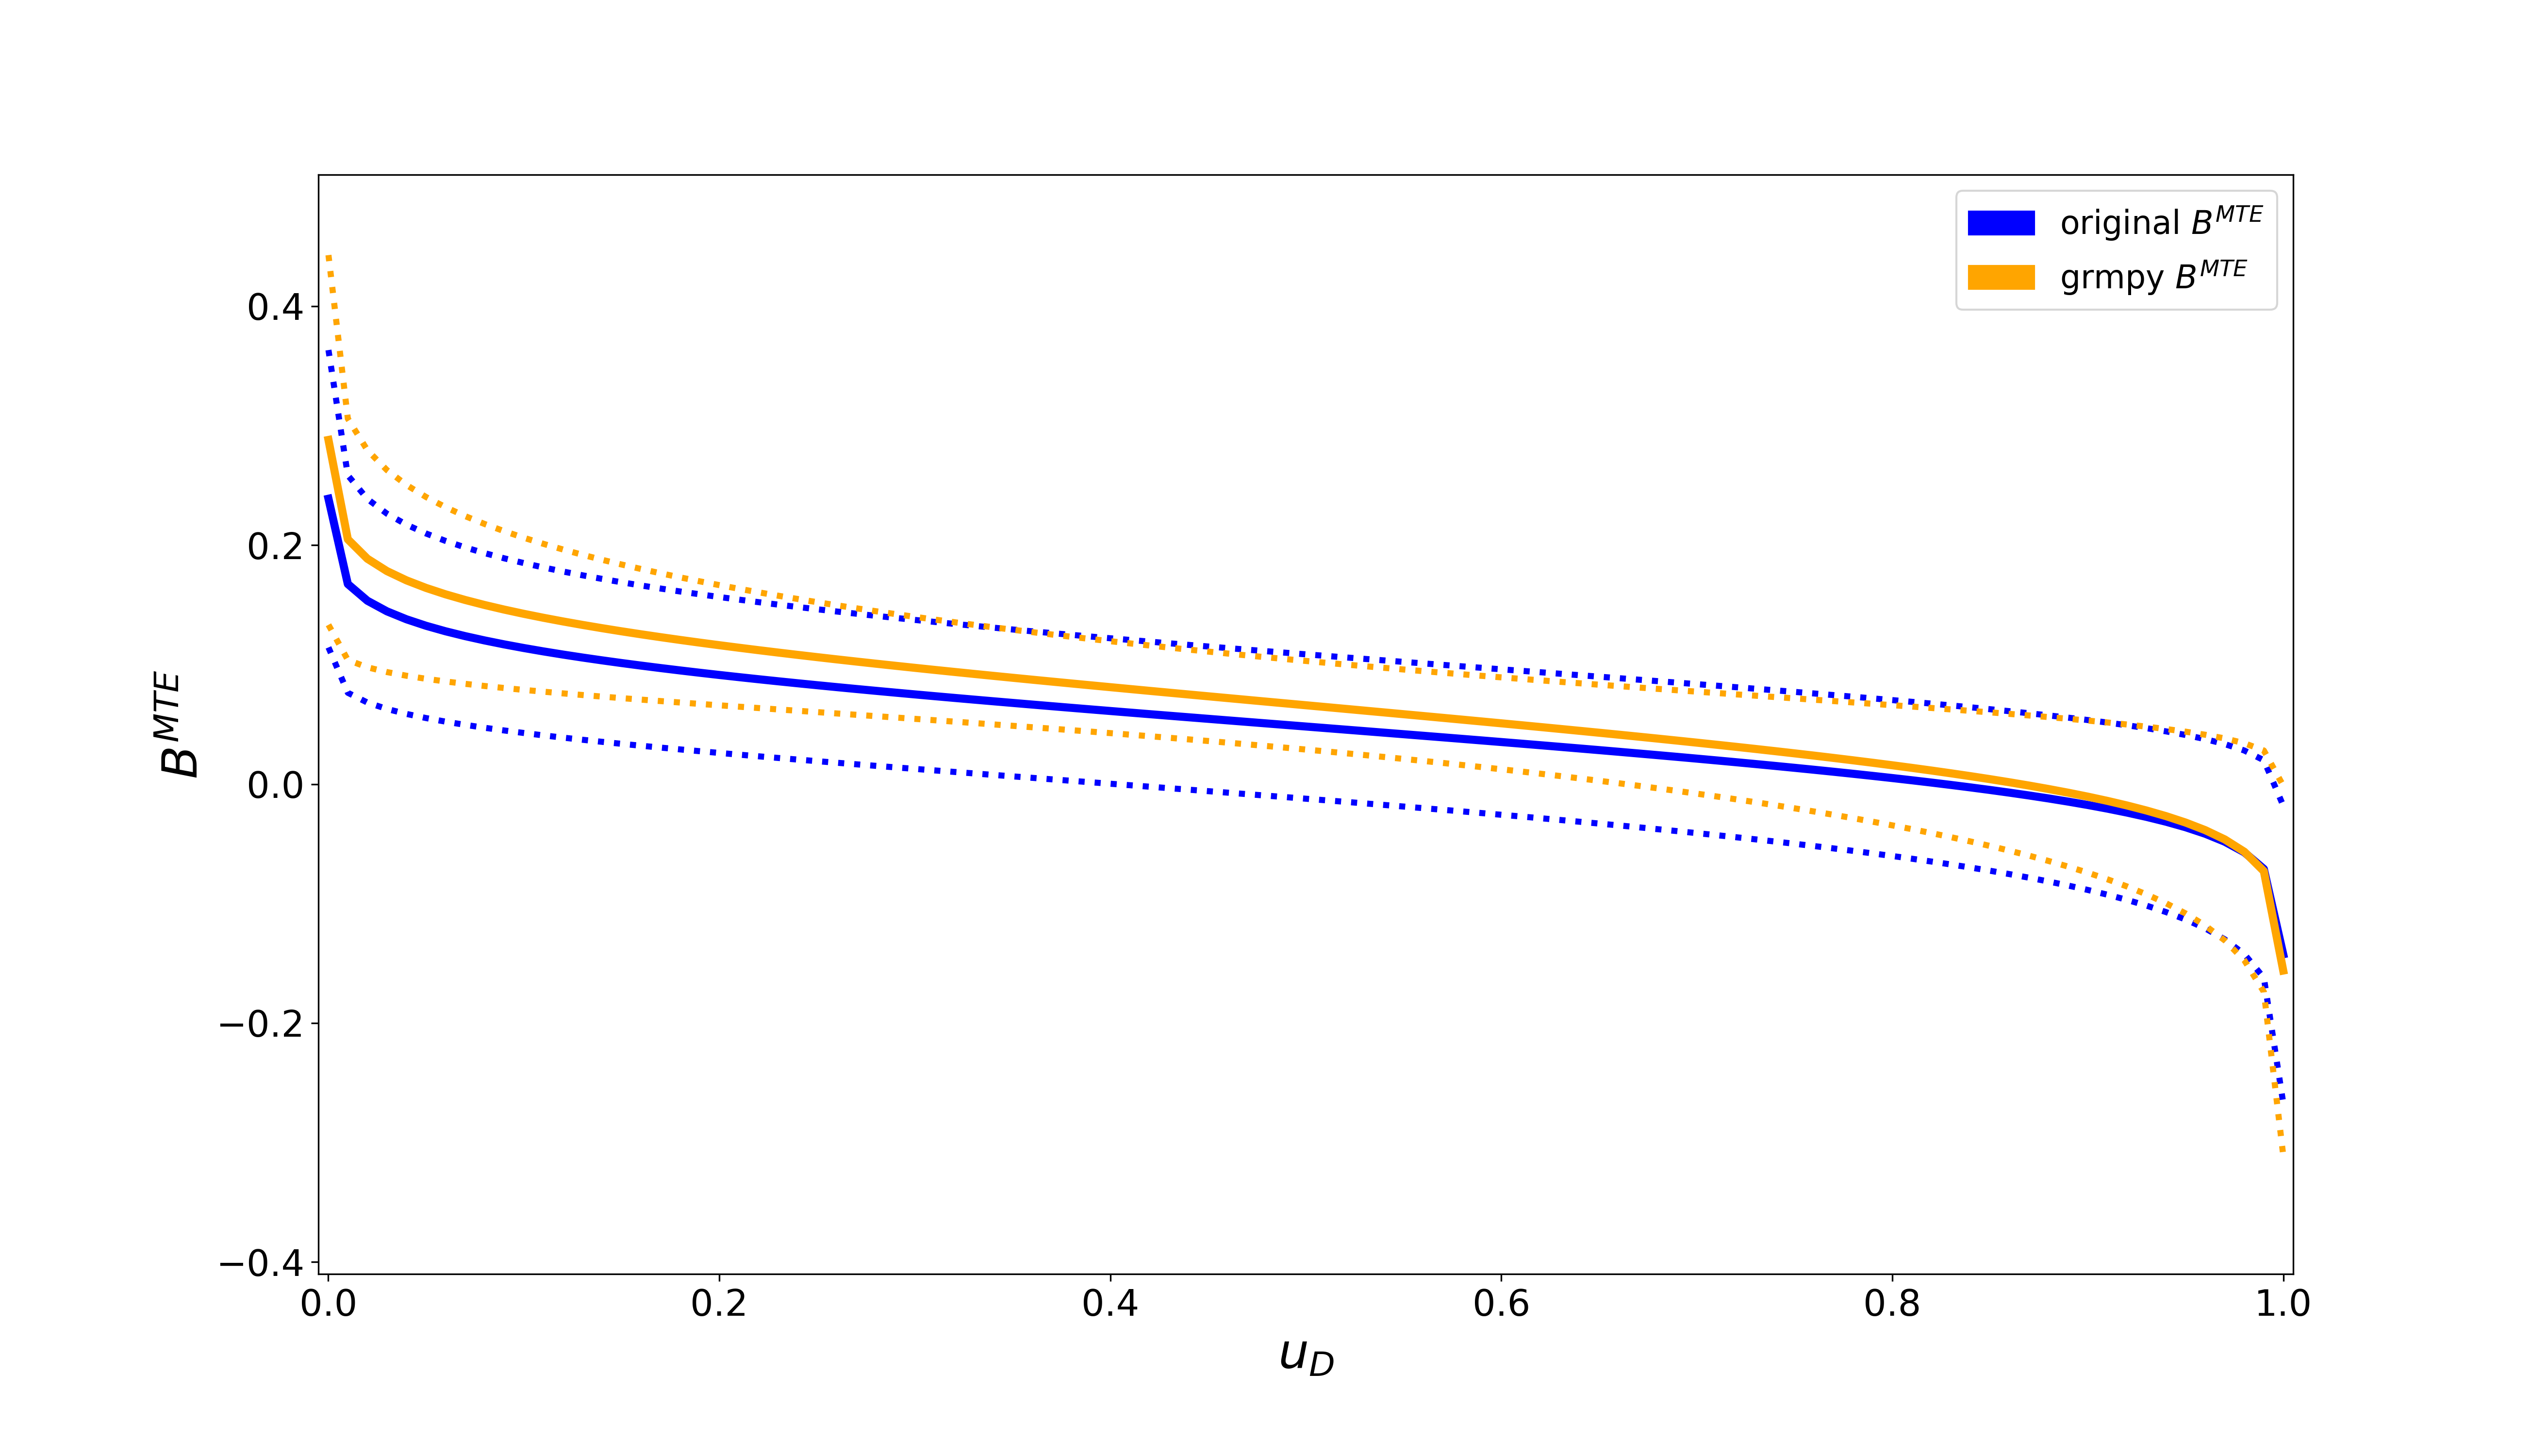
\includegraphics[width=110mm]{figures/fig-marginal-benefit-parametric-replication.png}
  \end{figure}
\end{frame}

\begin{frame}
\begin{figure}
  \caption{Performance comparison}
  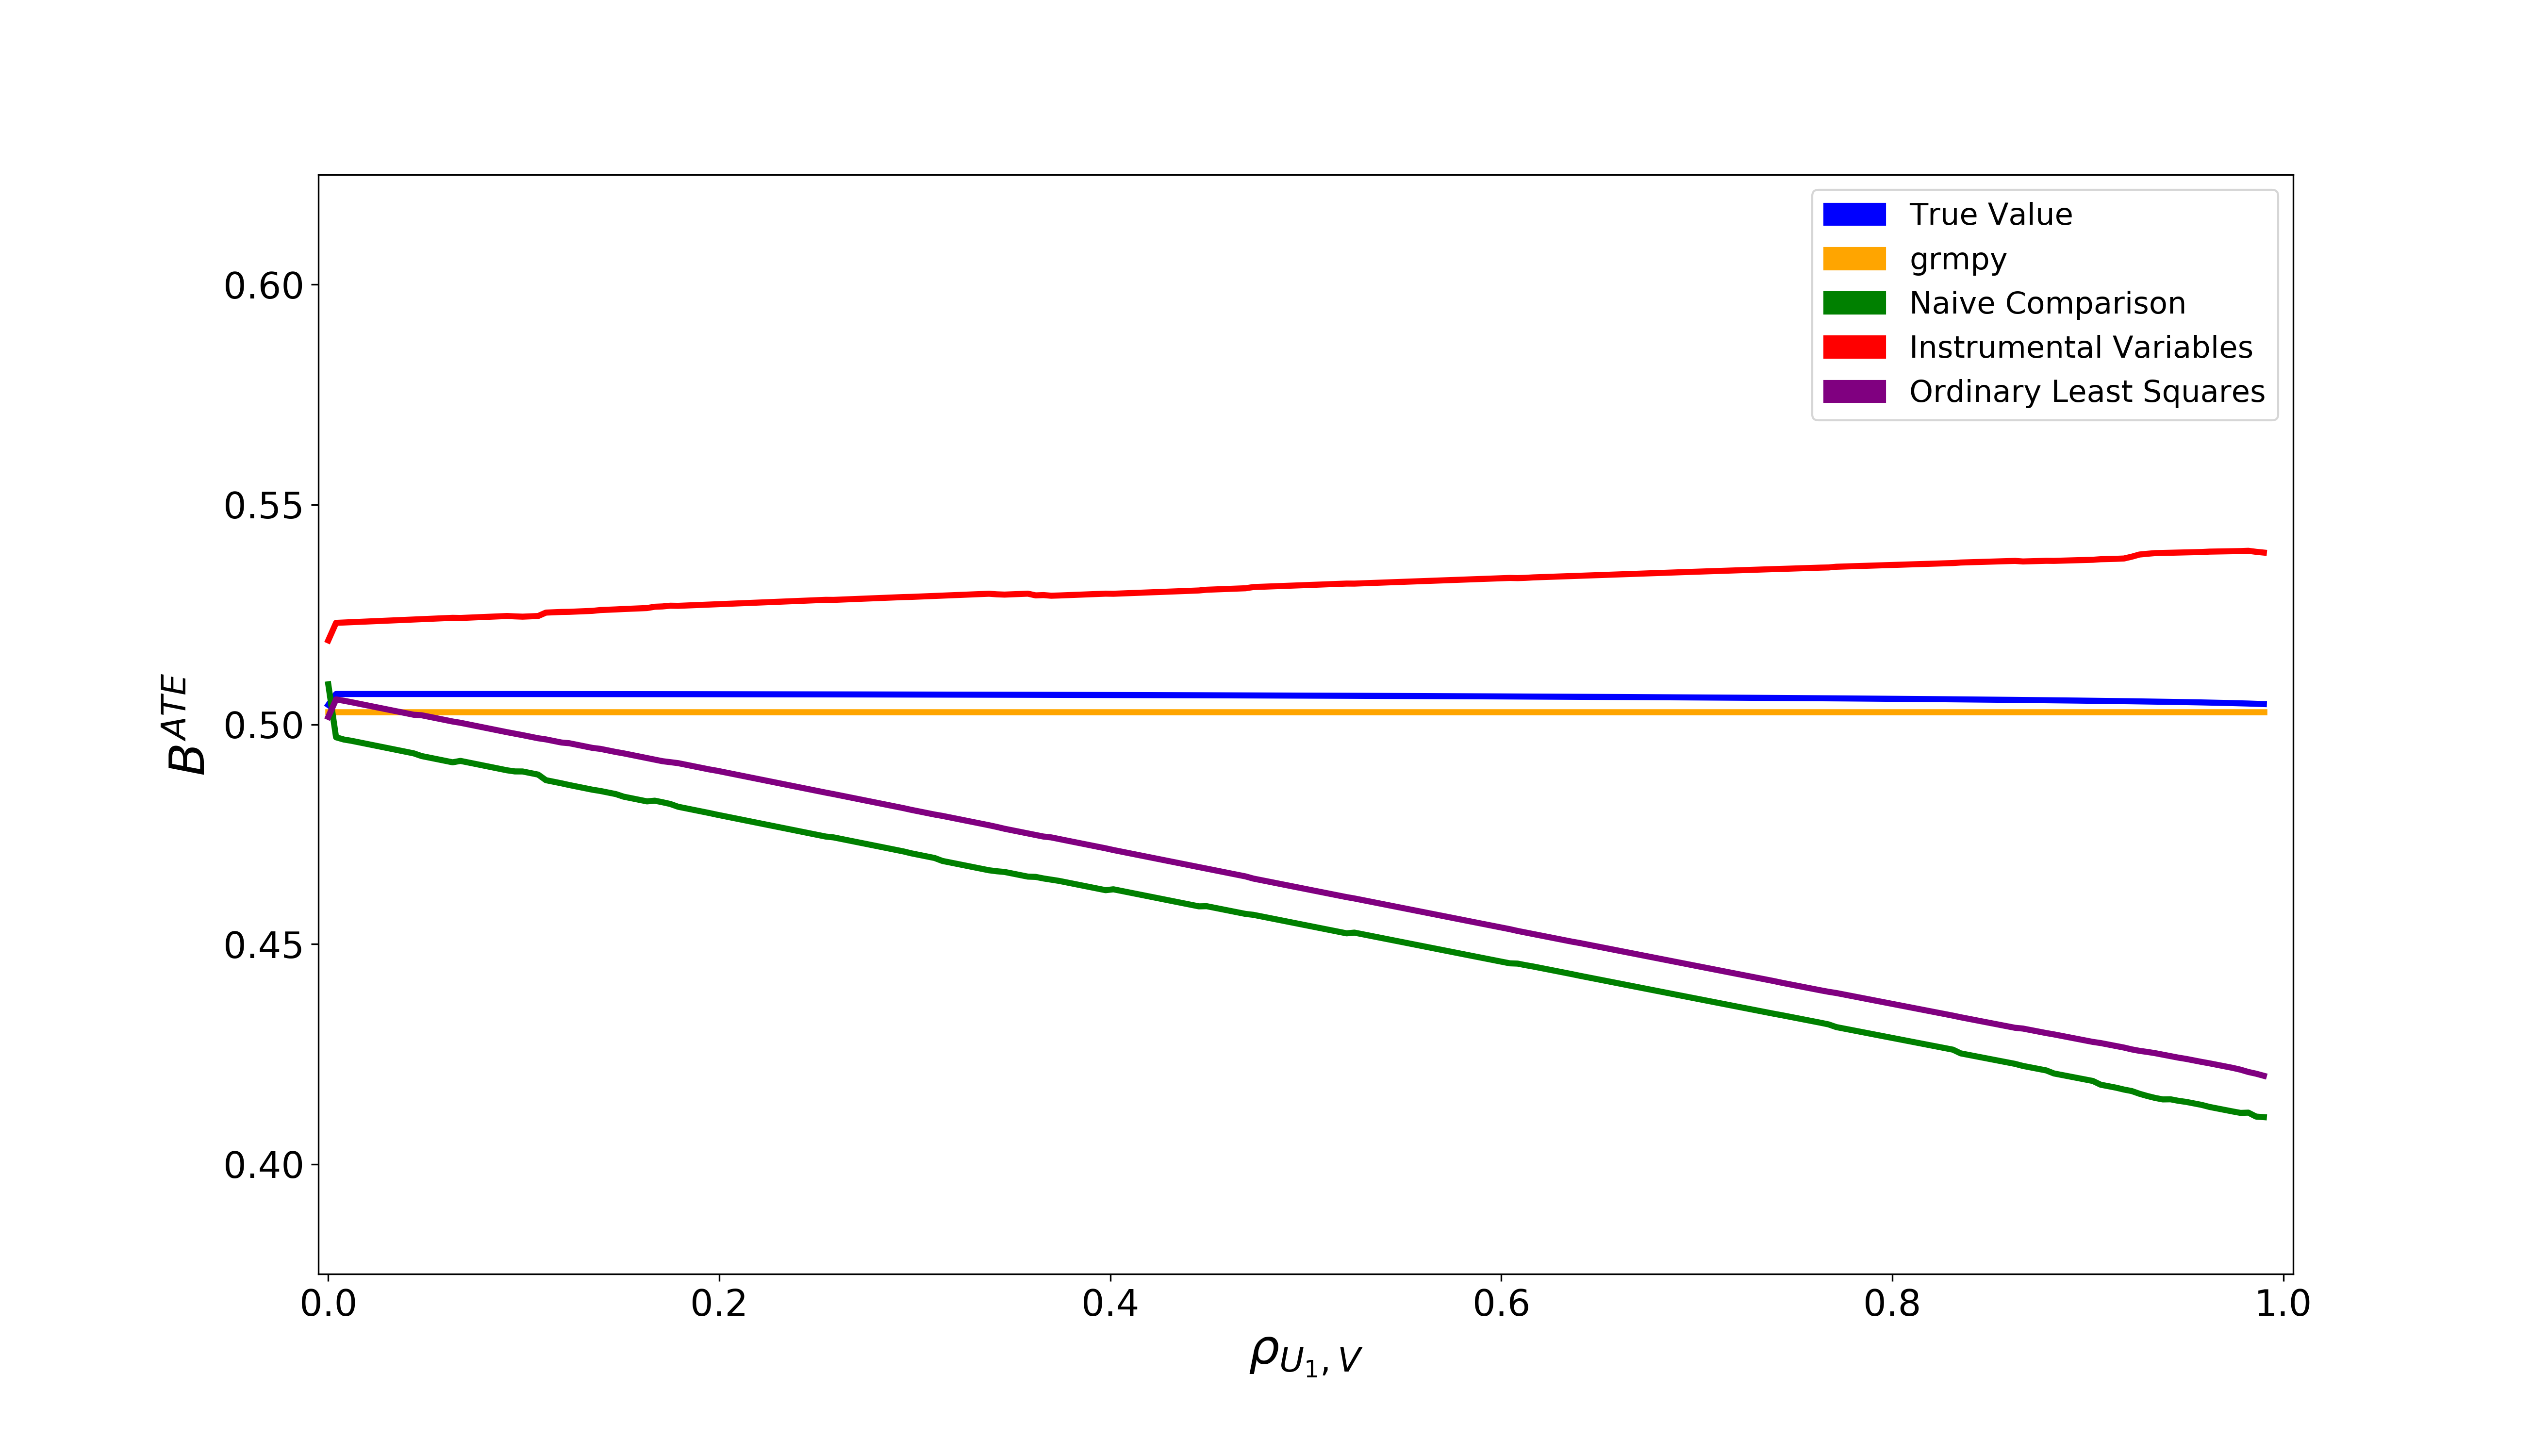
\includegraphics[width=110mm]{figures/fig1.png}
\end{figure}


\end{frame}

\begin{frame}
\textbf{Implementation of standard errors and adjustments on the output files}
\vfill
\begin{center}
See: \href{examples/est.grmpy.info}{Example}
\end{center}
\vfill
\end{frame}

\begin{frame}
\textbf{Online documentation}
\vfill
\begin{figure}
  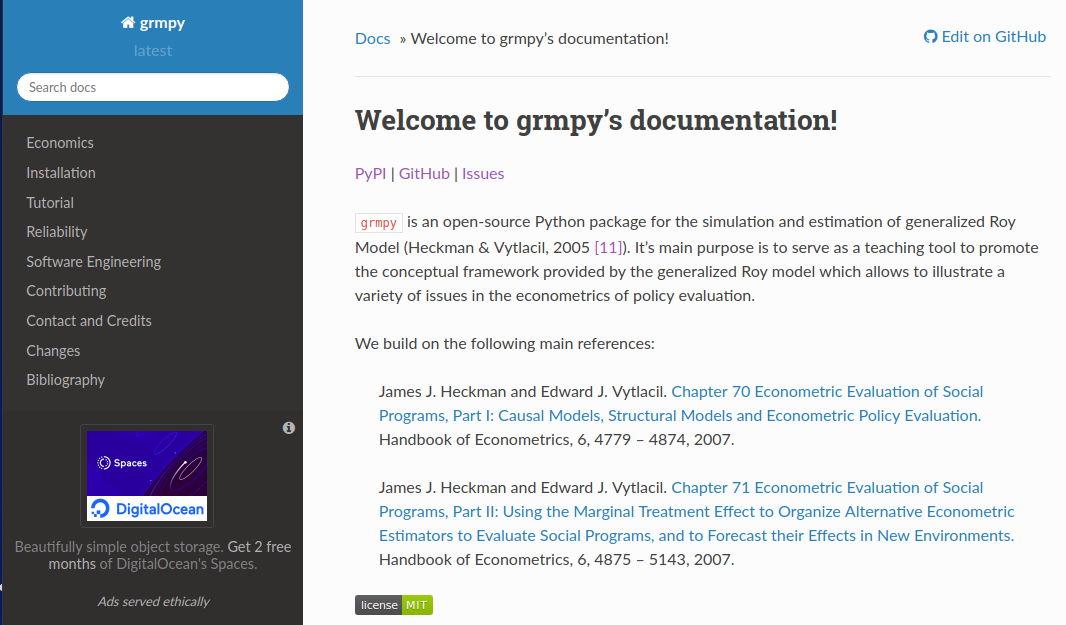
\includegraphics[scale=0.3]{figures/docu.png}
\end{figure}
\vfill
\end{frame}
